\begin{pastexam}[label={px:ntu-110-comm-dsa-41}]{臺大電信所 110 學年度（B）第 41 題}
（複選；每題 2.5 分，每答錯一個選項倒扣 0.5 分至該題 0 分止）

In this exam,
\begin{itemize}
\item The height of a leaf (in either a tree or heap) is defined as 0.
\item The depth of the root (in either a tree or heap) is defined as 0.
\item The degree of a node (in either a tree or heap) is defined as the number of its children.
\item The size of a tree/heap is defined as the total number of keys (items) it stores.
\item All heaps, unless otherwise specified, are min heaps.
\end{itemize}

Consider an AVL tree that results from successively inserting keys 2, 4, 5, 3, 8, 7, 1, 6, 9 into an initially empty tree. Which of the following statements are true?
\begin{enumerate}[label=\Alph*.]
\item The tree height is 4.
\item Key 3 and key 5 have the same depth.
\item Key 2 and key 8 have the same height.
\item Key 6 is a leaf.
\item Key 7 is the parent of key 9.
\end{enumerate}
\end{pastexam}

\begin{pastsoln}
答案是 B、C、D。

依序插入，每次插入後從新節點往上找第一個失衡（左右高度差 $2$）的節點旋轉（資結書第~10.2.3~節）：
\begin{itemize}
\item 插入 $2, 4$：$2$ 的右子節點 $4$。
\item 插入 $5$：$2$ 失衡（右子樹高、新鍵在右的右），RR 型，對 $2$ 左旋，根變成 $4$，子節點 $2, 5$。
\item 插入 $3$：放 $2$ 的右。 插入 $8$：放 $5$ 的右。 都沒有失衡。
\item 插入 $7$：放 $8$ 的左。 $5$ 失衡（右邊高 $2$），新鍵在右子樹的左邊，RL 型：先對 $8$ 右旋、再對 $5$ 左旋，
$7$ 上來，子節點 $5, 8$。
\item 插入 $1$：放 $2$ 的左。 插入 $6$：$>4$、$<7$、$>5$，放 $5$ 的右；$7$ 的左右高度是 $1$ 和 $0$，$4$ 的是 $1$ 和
$2$，都沒失衡。
\item 插入 $9$：放 $8$ 的右，沒有失衡。
\end{itemize}
\begin{center}
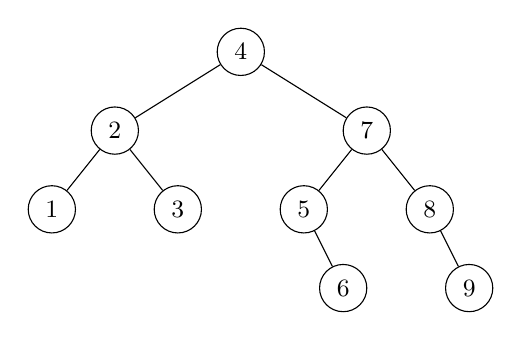
\begin{tikzpicture}[every node/.style={circle,draw,inner sep=1pt,minimum size=6mm,font=\small},level distance=10mm,edge from parent/.style={draw},level 1/.style={sibling distance=32mm},level 2/.style={sibling distance=16mm},level 3/.style={sibling distance=10mm}]
\node {4}
  child {node {2} child {node {1}} child {node {3}}}
  child {node {7}
    child {node {5} child[missing] child {node {6}}}
    child {node {8} child[missing] child {node {9}}}};
\end{tikzpicture}
\end{center}
\begin{itemize}
\item A 錯：最長路徑 $4 \to 7 \to 5 \to 6$，$3$ 條邊，樹高 $3$。
\item B 對：$3$ 是 $4 \to 2 \to 3$，$5$ 是 $4 \to 7 \to 5$，深度都是 $2$。
\item C 對：$2$ 的子節點 $1, 3$ 都是葉子，高度 $1$；$8$ 只有葉子 $9$，高度也是 $1$。
\item D 對：$6$ 沒有子節點。
\item E 錯：$9$ 的父節點是 $8$。
\end{itemize}
\end{pastsoln}
